%%%%%%%%%%%%%%%%%%%%%%%%%%%%%%%%%%%%%%%%%
% Lachaise Assignment
% LaTeX Template
% Version 1.0 (26/6/2018)
%
% This template originates from:
% http://www.LaTeXTemplates.com
%
% Authors:
% Marion Lachaise & François Févotte
% Vel (vel@LaTeXTemplates.com)
%
% License:
% CC BY-NC-SA 3.0 (http://creativecommons.org/licenses/by-nc-sa/3.0/)
% 
%%%%%%%%%%%%%%%%%%%%%%%%%%%%%%%%%%%%%%%%%

%----------------------------------------------------------------------------------------
%	PACKAGES AND OTHER DOCUMENT CONFIGURATIONS

%----------------------------------------------------------------------------------------

\documentclass[UTF8]{ctexart}
\usepackage{verbatim} %for comments
\usepackage{ulem} % for English underline
\usepackage{xeCJKfntef} % for Chinese underline
\usepackage{subfigure} % 子图包
\usepackage{hyperref} %插入网址
%\usepackage{amsmath}
\usepackage{float}
\usepackage{graphicx}
%\usepackage[inkscapelatex=false]{svg}
%%%%%%%%%%%%%%%%%%%%%%%%%%%%%%%%%%%%%%%%%
% Lachaise Assignment
% Structure Specification File
% Version 1.0 (26/6/2018)
%
% This template originates from:
% http://www.LaTeXTemplates.com
%
% Authors:
% Marion Lachaise & François Févotte
% Vel (vel@LaTeXTemplates.com)
%
% License:
% CC BY-NC-SA 3.0 (http://creativecommons.org/licenses/by-nc-sa/3.0/)
% 
%%%%%%%%%%%%%%%%%%%%%%%%%%%%%%%%%%%%%%%%%

%----------------------------------------------------------------------------------------
%	PACKAGES AND OTHER DOCUMENT CONFIGURATIONS
%----------------------------------------------------------------------------------------

\usepackage{amsmath,amsfonts,stmaryrd,amssymb} % Math packages

\usepackage{enumerate} % Custom item numbers for enumerations

\usepackage[ruled]{algorithm2e} % Algorithms

\usepackage[framemethod=tikz]{mdframed} % Allows defining custom boxed/framed environments

\usepackage{listings} % File listings, with syntax highlighting
\lstset{
	basicstyle=\ttfamily, % Typeset listings in monospace font
}

%----------------------------------------------------------------------------------------
%	DOCUMENT MARGINS
%----------------------------------------------------------------------------------------

\usepackage{geometry} % Required for adjusting page dimensions and margins

\geometry{
	paper=a4paper, % Paper size, change to letterpaper for US letter size
	top=2.5cm, % Top margin
	bottom=3cm, % Bottom margin
	left=2.5cm, % Left margin
	right=2.5cm, % Right margin
	headheight=14pt, % Header height
	footskip=1.5cm, % Space from the bottom margin to the baseline of the footer
	headsep=1.2cm, % Space from the top margin to the baseline of the header
	%showframe, % Uncomment to show how the type block is set on the page
}

%----------------------------------------------------------------------------------------
%	FONTS
%----------------------------------------------------------------------------------------

\usepackage[utf8]{inputenc} % Required for inputting international characters
\usepackage[T1]{fontenc} % Output font encoding for international characters

\usepackage{XCharter} % Use the XCharter fonts

%----------------------------------------------------------------------------------------
%	COMMAND LINE ENVIRONMENT
%----------------------------------------------------------------------------------------

% Usage:
% \begin{commandline}
%	\begin{verbatim}
%		$ ls
%		
%		Applications	Desktop	...
%	\end{verbatim}
% \end{commandline}

\mdfdefinestyle{commandline}{
	leftmargin=10pt,
	rightmargin=10pt,
	innerleftmargin=15pt,
	middlelinecolor=black!50!white,
	middlelinewidth=2pt,
	frametitlerule=false,
	backgroundcolor=black!5!white,
	frametitle={Command Line},
	frametitlefont={\normalfont\sffamily\color{white}\hspace{-1em}},
	frametitlebackgroundcolor=black!50!white,
	nobreak,
}

% Define a custom environment for command-line snapshots
\newenvironment{commandline}{
	\medskip
	\begin{mdframed}[style=commandline]
}{
	\end{mdframed}
	\medskip
}

%----------------------------------------------------------------------------------------
%	FILE CONTENTS ENVIRONMENT
%----------------------------------------------------------------------------------------

% Usage:
% \begin{file}[optional filename, defaults to "File"]
%	File contents, for example, with a listings environment
% \end{file}

\mdfdefinestyle{file}{
	innertopmargin=1.6\baselineskip,
	innerbottommargin=0.8\baselineskip,
	topline=false, bottomline=false,
	leftline=false, rightline=false,
	leftmargin=2cm,
	rightmargin=2cm,
	singleextra={%
		\draw[fill=black!10!white](P)++(0,-1.2em)rectangle(P-|O);
		\node[anchor=north west]
		at(P-|O){\ttfamily\mdfilename};
		%
		\def\l{3em}
		\draw(O-|P)++(-\l,0)--++(\l,\l)--(P)--(P-|O)--(O)--cycle;
		\draw(O-|P)++(-\l,0)--++(0,\l)--++(\l,0);
	},
	nobreak,
}

% Define a custom environment for file contents
\newenvironment{file}[1][File]{ % Set the default filename to "File"
	\medskip
	\newcommand{\mdfilename}{#1}
	\begin{mdframed}[style=file]
}{
	\end{mdframed}
	\medskip
}

%----------------------------------------------------------------------------------------
%	NUMBERED QUESTIONS ENVIRONMENT
%----------------------------------------------------------------------------------------

% Usage:
% \begin{question}[optional title]
%	Question contents
% \end{question}

\mdfdefinestyle{question}{
	innertopmargin=1.2\baselineskip,
	innerbottommargin=0.8\baselineskip,
	roundcorner=5pt,
	nobreak,
	singleextra={%
		\draw(P-|O)node[xshift=1em,anchor=west,fill=white,draw,rounded corners=5pt]{%
		Question \theQuestion\questionTitle};
	},
}

\newcounter{Question} % Stores the current question number that gets iterated with each new question

% Define a custom environment for numbered questions
\newenvironment{question}[1][\unskip]{
	\bigskip
	\stepcounter{Question}
	\newcommand{\questionTitle}{~#1}
	\begin{mdframed}[style=question]
}{
	\end{mdframed}
	\medskip
}

%----------------------------------------------------------------------------------------
%	WARNING TEXT ENVIRONMENT
%----------------------------------------------------------------------------------------

% Usage:
% \begin{warn}[optional title, defaults to "Warning:"]
%	Contents
% \end{warn}

\mdfdefinestyle{warning}{
	topline=false, bottomline=false,
	leftline=false, rightline=false,
	nobreak,
	singleextra={%
		\draw(P-|O)++(-0.5em,0)node(tmp1){};
		\draw(P-|O)++(0.5em,0)node(tmp2){};
		\fill[black,rotate around={45:(P-|O)}](tmp1)rectangle(tmp2);
		\node at(P-|O){\color{white}\scriptsize\bf !};
		\draw[very thick](P-|O)++(0,-1em)--(O);%--(O-|P);
	}
}

% Define a custom environment for warning text
\newenvironment{warn}[1][Warning:]{ % Set the default warning to "Warning:"
	\medskip
	\begin{mdframed}[style=warning]
		\noindent{\textbf{#1}}
}{
	\end{mdframed}
}

%----------------------------------------------------------------------------------------
%	INFORMATION ENVIRONMENT
%----------------------------------------------------------------------------------------

% Usage:
% \begin{info}[optional title, defaults to "Info:"]
% 	contents
% 	\end{info}

\mdfdefinestyle{info}{%
	topline=false, bottomline=false,
	leftline=false, rightline=false,
	nobreak,
	singleextra={%
		\fill[black](P-|O)circle[radius=0.4em];
		\node at(P-|O){\color{white}\scriptsize\bf i};
		\draw[very thick](P-|O)++(0,-0.8em)--(O);%--(O-|P);
	}
}

% Define a custom environment for information
\newenvironment{info}[1][Info:]{ % Set the default title to "Info:"
	\medskip
	\begin{mdframed}[style=info]
		\noindent{\textbf{#1}}
}{
	\end{mdframed}
}
 % Include the file specifying the document structure and custom commands

%----------------------------------------------------------------------------------------
%	ASSIGNMENT INFORMATION
%----------------------------------------------------------------------------------------

\title{NLP数学基础:数学分析} % Title of the assignment

\author{Zyf\\ \texttt{ahhuer@163.com}} % Author name and email address

\date{Hohai University--- \today} % University, school and/or department name(s) and a date

%----------------------------------------------------------------------------------------

\begin{document}

\maketitle % Print the title

%----------------------------------------------------------------------------------------
%	INTRODUCTION
%----------------------------------------------------------------------------------------

\section*{基本介绍Introduction} % Unnumbered section

\textbf{数学分析学},也称\textbf{分析数学}、\textbf{分析学}或\textbf{解析学}(Mathematical Analysis),是普遍存在于大学数学专业的一门基础课程。大致与非数学专业学生的高等数学课程内容相近,但内容更加深入,一般指以微积分学、无穷级数和解析函数等的一般理论为主要内容,并包括它们的理论基础的一个较为完整的数学学科。

数学分析研究的内容包括\textbf{实数、复数、实函数及复变函数}。数学分析是由微积分演进而来,在微积分发展至现代阶段中,从应用中的方法总结升华为一类综合性分析方法,且初等微积分中也包括许多数学分析的基础概念及技巧,可以认为这些应用方法是高等微积分生成的前提。数学分析的方式和其几何有关,不过只要任一数学空间有定义邻域(拓扑空间)或是有针对两物件距离的定义(度量空间),就可以用数学分析的方式进行分析。


\begin{info} % Information block
	本项目只是简单总结数学分析中的一些基础知识(AI需要用到的基础知识):数列极限、函数极限、微积分、多元微积分......,要想系统学习数学分析,可以参考另外的教材进行更加深入的学习。
\end{info}

%----------------------------------------------------------------------------------------
%	PROBLEM 1
%----------------------------------------------------------------------------------------

\section{数列极限Sequence Limit} % Numbered section

\textbf{数列}是一列两个以上按顺序排列的数,所组成的序列,一般记作\( \{ a_k\}_{k=1}^{\infty} \)或\( \{ a_l\}_{l=1}^{n} \),分别表示无穷数列和有限数列(个数为$n$)。数列中的每一个数称为这个数列的“\textbf{项}”。$a_1$为数列的“第一项”、$a_2$为“第二项”、 $a_n$则为“第$n$项”。项的总个数为数列的“\textbf{项数}”。数列中的第一项常称为“\textbf{首项}”,最后一项则称为“\textbf{末项}”,这里所有$n \in \text{N}^{+}$。
\begin{info}[Notice:] % Information block
	数列不仅仅可以分成有限数列和无穷数列,还有以下两种常见类型:
	\begin{enumerate}
		\item{\textbf{有界数列}}\\
		 $\blacktriangleright$ 若对所有\( n \in \text{N}^{+} \),\( \exists M, N \in \text{R} \),使得\( M \leqslant a_n \leqslant N \),则称数列$\{ a_n \}$为“\textbf{有界数列}”。 $ M $称为“\textbf{下界}”,$ N $称为“\textbf{上界}”。\\
         $\blacktriangleright$若对数列$\{ a_n \}$,上述的$ M $ 、$ N $不存在,则称数列$\{ a_n \}$为“\textbf{无界数列}”。
		\item{\textbf{单调数列}}\\
		$\blacktriangleright$ 若对所有\( n \in \text{N}^{+} \),\( a_{n+1} \geqslant a_n \) ,则称数列$\{ a_n \}$为“\textbf{递增数列}”。把 $\geqslant$ 换成 $>$ ,则称为“\textbf{严格递增数列}”。\\
        $\blacktriangleright$若对所有\( n \in \text{N}^{+} \),\( a_{n+1} \leqslant a_n \) ,则称数列$\{ a_n \}$为“\textbf{递减数列}”。把 $\leqslant$ 换成 $<$ ,则称为“\textbf{严格递减数列}”。\\
        $\blacktriangleright$若对所有\( n \in \text{N}^{+} \),\( a_{n+1} = a_n \) ,则称数列$\{ a_n \}$为“\textbf{常数数列}”。\\
	\end{enumerate}
\end{info}
%------------------------------------------------

\subsection{数列极限Sequence Limit}

一个关于数列很重要的性质是\textbf{收敛},如果一个数列收敛,它收敛到的东西便是它的极限值,一个数列收敛,那它便是收敛数列,否则为发散数列。

简单的说,一个数列$\{ x_n \}_{n=1}^{\infty}$有极限,便是它的数列中的元素逐渐地越来越靠近一个常数$L$(我们称$L$为数列$\{ x_n \}$的\textbf{极限值} ),但是它们仍然任意得很靠近极限值$L$,而不是真的等于。

\textbf{举例来说}:当\( x_n = \frac{1}{n} \)时,随着$n$的增加,可以看到$a_n$逐渐趋向于0。当$ x_n=5-\frac {3n^2-9}{n^2+1}$时,随着$n$的数字增加,可以看到它逐渐趋向于2。

此外,值得注意的是,当一个数列有极限值时,它的极限值一定是\textbf{唯一的}。一般来说,当数列$\{ x_n \}$收敛于常数$L$时,我们会记作:\( \lim_{n \to \infty} x_n = L\)。当$\{x_n\}$不收敛时,如:$\{x_n\}^{(1)}=(-1)^n$(极限不存在)、$\{x_n\}^{(2)}=n^2 \cdots$等这种极限\textbf{不存在}或者极限\textbf{无穷}的情况,我们称此数列\textbf{发散}。



% Numbered question, with subquestions in an enumerate environment
\begin{question}[\textbf{数列极限的严格定义是什么?}]
\textbf{定义(Def):}若数列$\{ x_n\}$有极限$a$,则对于任意给定的$ \varepsilon > 0$,存在正整数$\text{N}$,使得当$n > \text{N}$时,成立
\begin{equation}
  |x_n-a| < \varepsilon \text{,}
\end{equation}
则称数列$\{ x_n\}$收敛于$a$,记作
\begin{equation}
  \lim_{n \to \infty} x_n = a \text{,}
\end{equation}
如果不存在这样的实数$a$,则称数列$\{ x_n\}$发散。
\end{question}

\begin{info}[Notice:]其他概念\\
	$\blacktriangleright$在收敛的数列中,我们通常称极限为0的数列为\textbf{无穷小量}。\\
	$\blacktriangleright$\( \lim_{n \to \infty} x_n = a \Leftrightarrow \{x_n - a \} \)是无穷小量。
\end{info}
%------------------------------------------------

\subsection{数列极限的性质与定理Properties and Theorems}
\begin{enumerate}
	\item {\textbf{唯一性}}\\
	收敛数列的极限必唯一
	\item {\textbf{有界性}}\\
	收敛数列必有界
	\item {\textbf{保序性}}\\
	设数列$\{ x_n \}$,$\{  y_n \}$均收敛,若\( \lim_{n \to \infty} x_n = a \),\( \lim_{n \to \infty} y_n = b \),且$a<b$,则存在正整数$\text{N}$,当$n>\text{N}$时,成立$x_n < y_n$
	\item {\textbf{夹逼性}}\\
	若三个数列$\{ x_n \}$,$\{  y_n \}$,$\{  z_n \}$从某项开始成立,
	\begin{equation}
		x_n \leqslant y_n \leqslant z_n \text{,} n>\text{N}_0
	\end{equation}
	且\( \lim_{n \to \infty} x_n = a \),\( \lim_{n \to \infty} z_n = a \),则\( \lim_{n \to \infty} y_n = a \)
	\item {\textbf{单调有界数列必有极限}}
\end{enumerate}

% 下面的格式可以用于阐述多行注释
\begin{comment}% 多行注释
	\begin{center}
	\begin{minipage}{0.5\linewidth} % Adjust the minipage width to accomodate for the length of algorithm lines
		\begin{algorithm}[H]
			\KwIn{$(a, b)$, two floating-point numbers}  % Algorithm inputs
			\KwResult{$(c, d)$, such that $a+b = c + d$} % Algorithm outputs/results
			\medskip
			\If{$\vert b\vert > \vert a\vert$}{
				exchange $a$ and $b$ \;
			}
			$c \leftarrow a + b$ \;
			$z \leftarrow c - a$ \;
			$d \leftarrow b - z$ \;
			{\bf return} $(c,d)$ \;
			\caption{\texttt{FastTwoSum}} % Algorithm name
			\label{alg:fastTwoSum}   % optional label to refer to
		\end{algorithm}
	\end{minipage}
\end{center}
\end{comment}


%----------------------------------------------------------------------------------------
%	PROBLEM 2
%----------------------------------------------------------------------------------------

\section{函数极限}

在数学中,\textbf{函数极限}是微积分学和数学分析的一个基本概念。它描述函数值在接近某一给定的自变量时的特征。

不严格地讲,函数$f$对于每个给定的在定义域内自变量,都会有一个对应的因变量$f(x)$。声称在自变量为p时,函数极限为$A$则表明:当自变量$x$的值无限接近于$p$时,因变量$f(x)$的值便无限接近于$A$。另一方面,如果存在十分接近于$p$的自变量所对应的因变量的值与$A$的值相差较大,则表示函数极限不存在。

极限的概念在现代微积分领域用途良多。比如,\textbf{连续性的定义}、\textbf{导数的定义}......
\begin{question}[\textbf{函数极限的严格定义是什么?}]
\textbf{定义(Def):}设函数$f(x)$在$x_0$的某一去心邻域有定。如果存在常数$A$,对于任意给定的$\varepsilon > 0$,存在$\delta > 0$,使得当$0 < |x-x_0| < \delta$时,成立
\begin{equation}
  |f(x)-A| < \varepsilon \text{,}
\end{equation}
则称函数$f(x)$收敛于$A$,记作
\begin{equation}
  \lim_{x \to x_0} f(x) = A \text{ 或 \ }f(x) \to A(x \to x_0)
\end{equation}
\end{question}

\begin{info}[Notice:]函数的左极限和右极限的定义:
\begin{enumerate}
	\item \textbf{左极限}\\
	$\blacktriangleright$只需要将上述函数极限的定义中$0 < |x-x_0| < \delta$修改为$-\delta < x-x_0 < 0$,即有:\( \lim_{x \to x_0^{-}} f(x) = A  \text{ 或 \ }f(x) \to A (x \to x_0^{-})\)
	\item \textbf{右极限}\\
	$\blacktriangleright$只需要将上述函数极限的定义中$0 < |x-x_0| < \delta$修改为$0 < x-x_0 < \delta$,即有:\( \lim_{x \to x_0^{+}} f(x) = A \text{ 或 \ }f(x) \to A (x \to x_0^{+})\)
\end{enumerate}
\end{info}
%------------------------------连续函数Continuous Function------------------------------
\subsection{连续函数Continuous Function}
\textbf{连续函数}(Continuous Function)是指函数在数学上的属性为连续。直观上来说,连续的函数就是当输入值的变化足够小的时候,输出的变化也会随之足够小的函数。

如果输入值的某种微小的变化会产生输出值的一个突然的跳跃甚至无法定义,则这个函数被称为是\textbf{不连续函数},或者说具有\textbf{不连续性}。直观上看,非连续函数一定存在间断点。

举例来说,考虑描述一棵树的高度随时间而变化的函数$h(t)$,那么这个函数是连续的(除非树被砍断)。又例如,假设{$T(P)$表示地球上某一点$P$的空气温度,则这个函数也是连续的。\textbf{事实上,古典物理学中有一句格言:“自然界中,一切都是连续的。”}相比之下,如果$M(t)$表述在时间$t$的时候银行账户上的钱币金额,则这个函数无论在存钱或者取钱的时候都会有跳跃,因此函数$M(t)$是不连续的。
\begin{question}[\textbf{函数连续的严格定义是什么?}]
\textbf{定义(Def):}考虑函数\( f : \mathbf{I} \longrightarrow \mathbf{J} \)。假设$c$是$f$的定义域中的元素。函数$f$被称为是在$c$点连续当且仅当以下条件成立:
\begin{quote}
	对于任意的正实数$ \varepsilon >0 $,存在一个正实数$\delta >0$使得对于任意定义域中的$x \in \mathbf{I}$,只要$x$满足\( c-\delta <x<c+\delta  \),成立
\begin{equation}
  |f(x)-f(c)| < \varepsilon \text{,}
\end{equation}
\end{quote}
则称函数$f(x)$在$c$点连续,记作\( \lim_{x \to c} f(x) = f(c) \text{ 或 \ }f(x) \to f(c) (x \to c)\)
\end{question}

\begin{info}[Notice:]\textbf{连续函数的性质}\\
	$\blacktriangleright$如果两个函数$f$和$g$是连续的,$ \lambda $为一个实数,那么$ f+g $、$\lambda f$和$ f \cdot g $都是连续的。如果对于定义域内的所有$x$,都有$g(x) \neq 0$,那么$\frac{f}{g}$也是连续的。\textbf{所有连续函数的集合构成一个环,也构成一个向量空间}(实际上构成一个代数)。\\
    $\blacktriangleright$两个连续函数的复合函数$f \circ g$也是连续函数。\\
    $\blacktriangleright$如果实函数$f$在闭区间$[a, b]$内连续,且$k$是某个位于$f(a)$和$f(b)$之间的数,那么存在某个$[ a , b ]$内的数$c$,使得$f ( c ) = k$。这个定理称为\textbf{介值定理}。例如,如果一个小孩在五岁到十岁之间身高从1米增长到了1.5米,那么期间一定有某一个时刻的身高正好是1.3米。\\
    $\blacktriangleright$如果$f$在$[ a , b ]$内连续,且$f ( a ) \cdot f ( b ) < 0$,则中间一定有某一个点$c$,使得$f ( c ) = 0$,这个定理称为\textbf{零点存在定理},这是介值定理的一个推论。\\
    $\blacktriangleright$如果$f$在闭区间$[ a, b]$内连续,则它一定取得最大值,也就是说,总存在$c \in [ a, b]$,使得对于所有的$x \in [ a, b]$,有$ f ( c ) \geqslant f(x)$。同样地,函数也一定有最小值。这个定理称为\textbf{极值定理}。(注意如果函数是定义在开区间$( a, b)$内,则它不一定有最大值和最小值,例如定义在开区间$(0,1)$内的函数$f ( x ) = \frac{1}{x}$。)
\end{info}
%---------------------------一致连续函数Uniformly Continuous----------------------------
\subsection{一致连续函数Uniformly Continuous}
\textbf{一致连续}又称\textbf{均匀连续}(Uniformly Continuous),为数学分析的专有名词,大致来讲是描述对于函数$f$我们只要在定义域中让任意两点$x$跟$y$越来越接近,我们就可以让$f(x)$跟$f(y)$无限靠近,这跟一般的连续函数不同之处在于:$f(x)$跟$f(y)$之间的距离并不依赖$x$跟$y$的位置选择。一致连续是比连续更苛刻的条件。一个函数在某\textbf{度量空间}上一致连续,则其在此\textbf{度量空间}上必然连续,但反之未必成立。

\begin{question}[\textbf{函数一致连续的严格定义是什么?}]
	当 $X$和$Y$都是实数的子集合,函数$f:X\to Y$在区间$I \in X$上一致连续的定义可表述为:如果对任意的$\varepsilon >0$,存在$\delta >0$,使得对任意两点$x\text{,}y \in I$满足$|x-y|<\delta$,都有
\begin{equation}
	|f(x)-f(y)|<\varepsilon \text{,}
\end{equation}
则称函数$f$在$I$上一致连续。\\
$\divideontimes$ \textbf{一致连续跟在每点连续最大的不同在于:在一致连续定义中,正数$\delta$的选择只依赖$\varepsilon$变量,而不依赖定义域上点的位置。}
\end{question}

\begin{info}[Notice:]\textbf{一致连续函数和非一致连续函数的例子}
\begin{enumerate}
	\item \textbf{一致连续函数}\\
		正弦三角函数$f(x)=sinx$、余弦三角函数$f(x)=cosx$、在规定区间上的多项式函数$f(x)=x^2\text{,}x \in [0, \rho] \cdots$ 
	\item \textbf{非一致连续函数}\\
		在无穷区间上的多项式函数$f(x)=x^2\text{,}x \in [0, +\infty)$、$f(x)=\frac{1}{x}\text{,}x \in (0, 1) \cdots$
\end{enumerate}
\end{info}
%-------------------------------一阶导数与微分Derivative--------------------------------
\subsection{一阶导数与微分Derivative}
	\textbf{导数}(Derivative)是\textbf{微积分}学中重要的基础概念。函数在某一点的导数是指这个函数在这一点附近的\textbf{变化率}。
	
	\textbf{导数的本质是通过极限的概念对函数进行局部的线性逼近}。当函数$f$的自变量在一点$x_0$上产生一个增量$h$时,函数输出值的增量与自变量增量$h$的比值在$h$趋于0时的极限如果存在,即为$f$在$x_0$处的导数,记作$f'(x_0)$、$\frac{\mathrm{d}f}{\mathrm{d}x}(x_0)$或$ \frac{\mathrm {d} f}{\mathrm {d} x}|_{x=x_0}$。
	
	例如在运动学中,物体的位移对于时间的导数就是物体的瞬时速度。
\begin{question}[\textbf{函数一阶导数的严格定义是什么?}]
	设有定义域和取值都在实数域中的函数 $y=f(x)$。若$f(x)$在点$x_0$的某个邻域内有定义,则当自变量 $x$在$x_0$处取得增量$\Delta x$(点 $x_{0}+\Delta x$仍在该邻域内)时,相应地$y$取得增量 $\Delta y=f(x_0+\Delta x)-f(x_0)$。如果$\Delta y$与$\Delta x$之比当$\Delta x\to 0 $时的极限存在,则称函数$y=f(x)$在点$x_0$处\textbf{可导},并称这个极限为函数 $y=f(x)$在点$x_0$处的\textbf{导数},记为$f'(x_0)$,即
\begin{equation}
  f'(x_0)=\lim_{\Delta x \to 0} \frac{\Delta y}{\Delta x}=\lim_{\Delta x \to 0} \frac{f(x_0+\Delta x)-f(x_0)}{\Delta x}
\end{equation}
\end{question}

\subsubsection{导数的几何意义Geometric Meaning}
当函数定义域和取值都在实数域中的时候,导数可以表示函数的曲线上的切线斜率。如图所示:
\begin{figure}[H]
  \centering
  %requires \usepakege{graphics}
  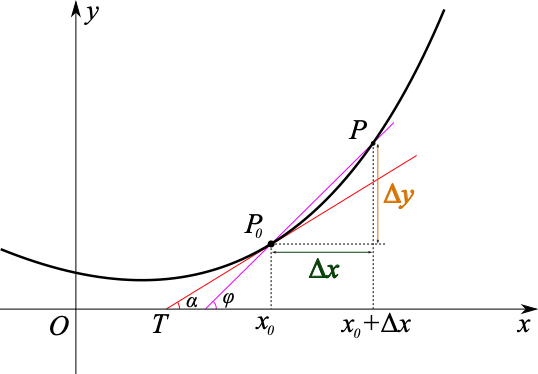
\includegraphics[scale=0.4]{Derivative.png}\\
  \caption{导数的几何意义}
\end{figure}

设$P_0$为曲线上的一个定点,$P$为曲线上的一个动点。当$P$沿曲线逐渐趋向于点$P_0$时,并且割线$PP_0$的极限位置$P_0T$存在,则称$P_0T$为曲线在$P_0$处的切线。

若曲线为一函数$y=f(x)$的图像,那么割线$PP_0$(紫色)的斜率为:
\begin{equation}
  \tan \varphi = \frac{\Delta y}{\Delta x}=\frac{f(x_0+\Delta x)-f(x_0)}{\Delta x}
\end{equation}

当$P_0$处的切线$P_0 T$(橘红色),即$P P_0$的极限位置存在时,此时$\Delta x \to 0$,$\varphi \to \alpha$,则$P_0 T$的斜率$\tan \alpha$为:
\begin{equation}
	\tan \alpha =\lim _{\Delta x\to 0} \tan \varphi =\lim _{\Delta x\to 0}\frac {f(x_{0}+\Delta x)-f(x_{0})}{\Delta x}
\end{equation}

上式与一般定义中的导数定义完全相同,也就是说$f'(x_0)=\tan \alpha$,因此,导数的几何意义即曲线$y=f(x)$在点$P_0(x_0,f(x_0))$处切线的\textbf{斜率}。

\begin{question}[\textbf{什么是微分?}]
	$\divideontimes$\textbf{微分}也是一种线性描述函数在一点附近变化的方式。微分和导数是两个不同的概念。但是,对一元函数来说,可微与可导是完全等价的。可微的函数,其微分等于导数乘以自变量的微分$\mathrm{d}x$,换句话说,函数的微分与自变量的微分之商等于该函数的导数。因此,导数也叫做\textbf{微商}。函数$y = f(x)$的微分又可记作$\mathrm{d}y = f'(x)\mathrm{d}x$。
\end{question}
\subsubsection{导数、导函数与微分算子}
若函数$f(x)$在其定义域包含的某区间$I$内每一个点都可导,那么也可以说函数$f(x)$在区间$I$内可导,这时对于$I$内每一个确定的$x$值,都对应着$f$的一个确定的导数值,如此一来就构成了一个新的函数$f'(x)$,这个函数称作原来函数$f(x)$的\textbf{导函数},记作:$y'$、$f'(x)$或者$\tfrac  {\mathrm {d}f}{\mathrm  {d}x}(x)$。

值得注意的是,\textbf{导数是一个数},是指函数$f(x)$ 在点$x_0$处导函数的函数值。但在不至于混淆的情况下,通常也可以说导函数为导数。
\begin{info}[Notice:]\textbf{“导数”补充知识点}\\
	$\blacktriangleright$导数是函数的局部性质。不是所有的函数都有导数,一个函数也不一定在所有的点上都有导数。如:$f(x)=|x|$在$x=0$处没有导数,但其他点都有导数。\\
    $\blacktriangleright$对于可导的函数$f$,$x \mapsto f'(x)$也是一个函数,称作$f$的导函数。寻找已知的函数在某点的导数或其导函数的过程称为\textbf{求导}。反之,已知导函数也可以倒过来求原来的函数,即不定积分。微积分基本定理说明了求原函数与积分是等价的。\textbf{求导和积分是一对互逆的操作},它们都是微积分学中最为基础的概念。
\end{info}
\begin{quote}
	如果一个函数的定义域为全体实数,即函数在$(-\infty,+\infty)$上都有定义,那么该函数是不是在定义域上处处可导呢?答案是否定的。函数在定义域中一点可导需要一定的条件。首先,要使函数$f$在一点可导,那么函数一定要在这一点处连续。换言之,\textbf{函数若在某点可导,则必然在该点处连续}。
\end{quote}

\begin{question}[\textbf{函数可导的条件是什么?}]
	\textbf{但仅仅是连续性并不能保证可导性}。即使函数在一点上连续,也不一定就在这一点可导。事实上,存在着在每一点都连续,但又在每一点都不可导的“\textbf{病态函数}”。1931年,\textbf{斯特凡·巴拿赫}甚至证明,事实上“绝大多数”的连续函数都属于这种病态函数。在连续而不可导的函数里,一种常见的情况是,函数在某一点连续,并且可以定义它的左导数和右导数:
\begin{eqnarray}
	\text{左导数:}f_{-}'(x_0)=\lim_{\Delta x \to 0^{-}}\frac{f(x_0+\Delta x)-f(x_0)}{\Delta x}\\
	\text{右导数:}f_{+}'(x_0)=\lim_{\Delta x \to 0^{+}}\frac{f(x_0+\Delta x)-f(x_0)}{\Delta x}
\end{eqnarray}
因此,\textbf{如果函数在一点的左右导数都存在并且相等,那么函数在该处可导}。
\end{question}


% Command-line "screenshot"
\begin{comment}
	\begin{commandline}
	\begin{verbatim}
		$ chmod +x hello.py
		$ ./hello.py

		Hello World!
	\end{verbatim}
\end{commandline}
\end{comment}


% Warning text, with a custom title
\begin{comment}
	\begin{warn}[Notice:]
  In congue risus leo, in gravida enim viverra id. Donec eros mauris, bibendum vel dui at, tempor commodo augue. In vel lobortis lacus. Nam ornare ullamcorper mauris vel molestie. Maecenas vehicula ornare turpis, vitae fringilla orci consectetur vel. Nam pulvinar justo nec neque egestas tristique. Donec ac dolor at libero congue varius sed vitae lectus. Donec et tristique nulla, sit amet scelerisque orci. Maecenas a vestibulum lectus, vitae gravida nulla. Proin eget volutpat orci. Morbi eu aliquet turpis. Vivamus molestie urna quis tempor tristique. Proin hendrerit sem nec tempor sollicitudin.
\end{warn}
\end{comment}

%----------------------------------------------------------------------------------------
%	PROBLEM 3
%----------------------------------------------------------------------------------------

\section{不定积分与定积分Integral}
\textbf{积分}(Integral)是微积分学与数学分析里的一个核心概念。通常分为\textbf{定积分}和\textbf{不定积分}两种。直观地说,对于一个给定的正实值函数$f(x)$,$f(x)$在一个实数区间$[a,b]$上的定积分
\begin{equation}
	\int _{a}^{b}f(x)\,\mathrm {d} x
\end{equation}
可以在数值上理解为在$ \textstyle Oxy$坐标平面上,由曲线$(x,f(x))(x\in [a,b])$,直线$x=a\text{,}x=b$以及$x$轴围成的曲边梯形的面积值(一种确定的实数值)。

$f(x)$的\textbf{不定积分}(或\textbf{原函}数)是指任何满足导数是函数$f(x)$的函数$F(x)$。一个函数$f(x)$的不定积分不是唯一的:只要$F(x)$是$f(x)$的不定积分,那么与之相差一个常数的函数 $F(x)+C$也是$f$的不定积分。

$\divideontimes$\underline{本项目中主要介绍\textbf{定积分},不定积分的介绍参见其它\textbf{数学分析教材}或者\textbf{维基百科}(Wikipedia)},
\underline{无说明的情况下,下文中的“积分”一词均指“定积分”。}
\begin{info}[Notice:]
定义积分的方法不止一种,各种定义之间也不是完全等价的。其中的差别主要是在定义某些特殊的函数:在某些积分的定义下这些函数不可积分,但在另一些定义之下它们的积分存在。然而有时也会因为教学的原因造成定义上的差别。最常见的积分定义是\textbf{黎曼积分}和\textbf{勒贝格积分}。我们主要探讨\textbf{黎曼积分}的由来与定义。
\end{info}

\textbf{黎曼积分}得名于德国数学家\textbf{波恩哈德·黎曼},建立在函数在区间取样分割后的黎曼和之上。
设有闭区间$[a,b]$,那么$[a,b]$的一个分割是指在此区间中取一个有限的点列$a=x_{0}<x_{1}<x_{2}<\ldots <x_{n}=b$。每个闭区间$[x_{i},x_{i+1}]$叫做一个\textbf{子区间}。定义$\lambda$为这些子区间长度的最大值:$\lambda =\max(x_{i+1}-x_{i})$,其中$0 \leqslant i \leqslant n-1$。而闭区间$[a,b]$上的一个取样分割是指在进行分割$a=x_{0}<x_{1}<x_{2}<\ldots <x_{n}=b$后,于每一个子区间中$[x_{i},x_{i+1}]$取出一点$x_{i}\leq t_{i}\leq x_{i+1}$。

对一个在闭区间$[a,b]$有定义的实值函数$f$,$f$关于取样分割$x_{0},\ldots ,x_{n}$、$t_{0},\ldots ,t_{n-1}$的\textbf{黎曼和}定义为以下和式:
\begin{equation}
	\sum _{i=0}^{n-1}f(t_{i})(x_{i+1}-x_{i})
\end{equation}
和式中的每一项是子区间长度$x_{i+1}-x_{i}$与在$t_{i}$处的函数值$f(t_{i})$的乘积。直观地说,就是以标记点$t_{i}$到$X$轴的距离为高,以分割的子区间为长的矩形的面积。下图是确定的子区间上不同的取样方式构成的黎曼和的不同效果图:
\begin{figure}[H]
  \centering
  %requires \usepakege{graphics}
  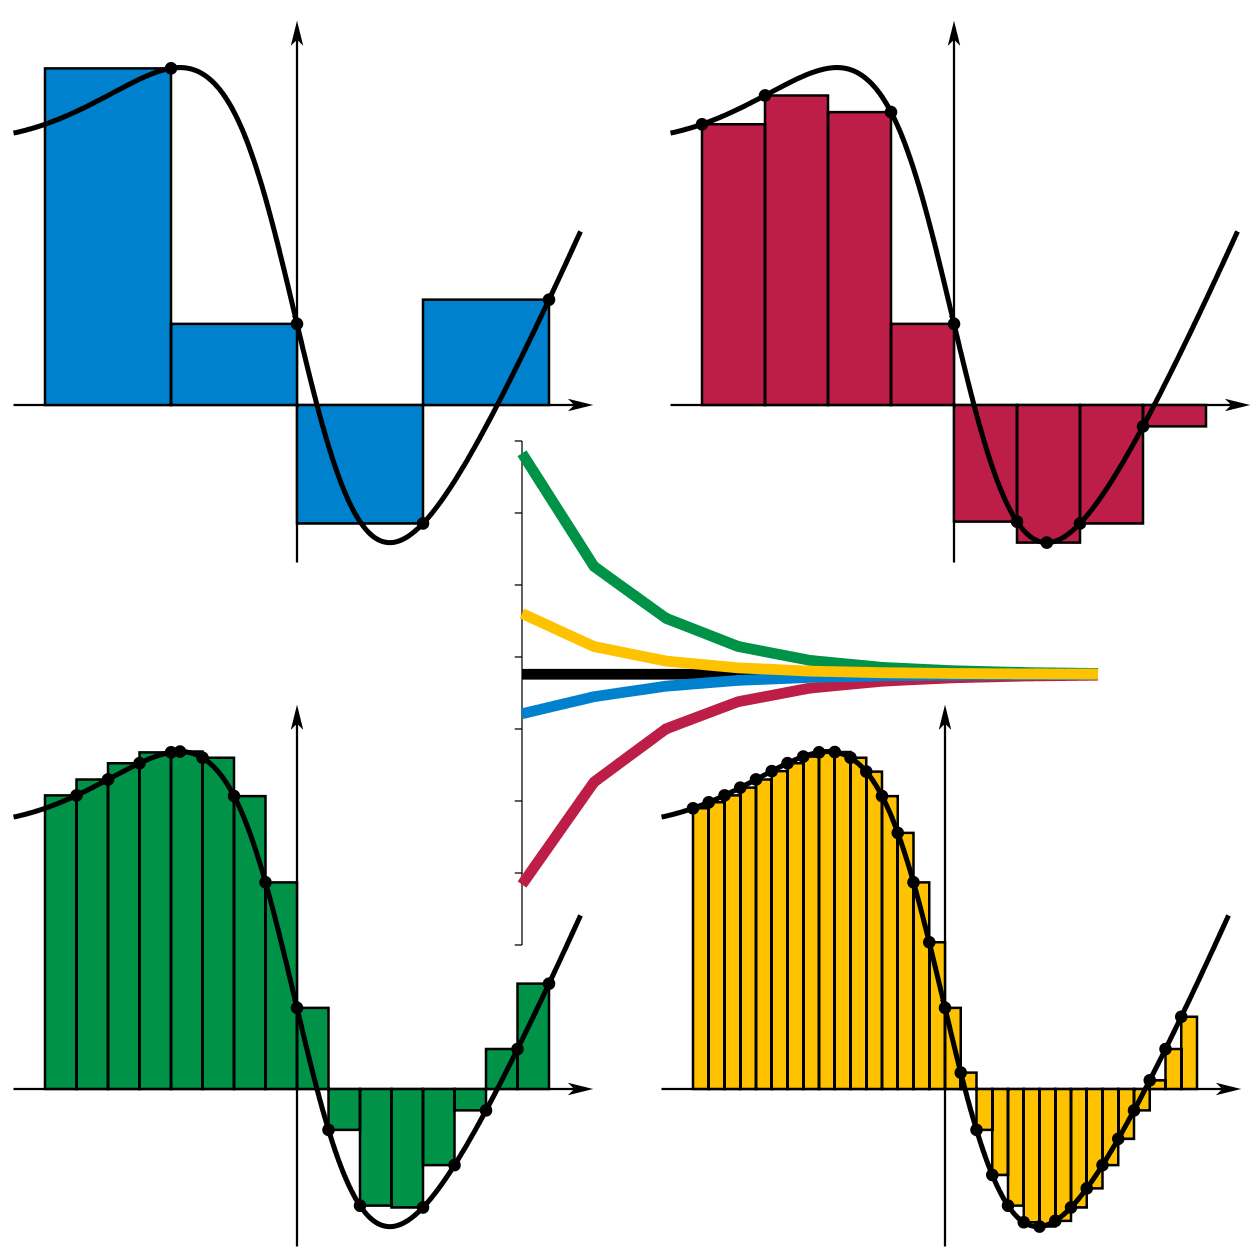
\includegraphics[scale=0.65]{Integral.png}\\
  \caption{左上:取右端值,右上:取极小值,左下:取极大值,右下:取左端值}
\end{figure}
最简单的取样分割方法是将区间均匀地分成若干个长度相等的子区间,然后在每个子区间上按相同的准则取得标记点。例如取每个子区间右端$t_i =x_{i+1}$(见图左上角)或者取每个子区间上函数的极大值对应的$t_{i}$(见图左下角)等等。不同的取样分割方式得到的黎曼和一般都不相同,而如果当$\lambda$足够小的时候,所有的黎曼和都趋于某个极限,那么这个极限就叫做函数$f$在闭区间$[a,b]$上的\textbf{黎曼积分}。即,$S$是函数$f$在闭区间$[a,b]$上的黎曼积分。
\begin{question}[\textbf{黎曼可积的严格定义是什么?}]
对于任意的$\varepsilon >0$,都存在$\delta >0$,使得对于任意的取样分割$P:a = x_{0} \leqslant x_1 \leqslant \ldots \leqslant x_{n}=b$以及$\forall t_{i} \in [x_i, x_{i+1}]$,只要它的子区间长度最大值$\lambda \leqslant \delta$,就有:
\begin{equation}
	\left|\sum _{i=0}^{n-1}f(t_{i})(x_{i+1}-x_{i})-S\right|<\varepsilon
\end{equation}
也就是说,对于一个函数$f$,如果在闭区间$[a,b]$上,无论怎样进行取样分割,只要它的子区间长度最大值足够小,函数$f$的黎曼和都会趋向于一个确定的值$S$,那么$f$在闭区间$[a,b]$上的黎曼积分存在,并且定义为黎曼和的极限$S$。这时候称函数$f$为黎曼可积的。将$f$在闭区间$[a,b]$上的黎曼积分记作:
\begin{equation}
	\int_a^b f(x) \mathrm{d} x
\end{equation}
\end{question}

\subsection{微积分基本定理Fundamental Theorem of Calculus}
\textbf{微积分基本定理}是将微分运算(求导运算)和积分运算(原函数)联系在一起的基本定理。从基本定理可以看出微分和积分运算之间的互逆关系。定理叙述如下:

\textbf{设有在闭区间$[a, b]$上连续的可积函数$f$。考虑积分上限函数$F(x) = \int_a^x f(t)\mathrm{d} t$,则$F$在闭区间$[a, b]$上连续,在开区间$(a, b)$上可导,并且对开区间$(a, b)$中任意的$x$有:}
\begin{equation}
	F'(x) = f(x)
\end{equation}
此定理表明:\textbf{给定任一连续函数,可以(利用积分)构造出该函数的反导函数。这一部分定理的重要之处在于它保证了连续函数的反导函数的存在性。}
\begin{info}[Notice:]微积分基本定理的一个实用的直接推论,也被称为\textbf{微积分第二基本定理}或是\textbf{牛顿-莱布尼茨公式:}
\begin{quote}
	设有在闭区间$[a,b]$上连续的可积函数$f$。考虑它的一个原函数$F(x)$,即:
\begin{equation}
	F'(x) = f(x)
\end{equation}
则$f$在区间$[a, b]$上的定积分满足:
\begin{equation}
	\int_a^b f(t) \mathrm{d} t = F(b) - F(a)
\end{equation}
\end{quote}
\end{info}
%----------------------------------------------------------------------------------------
%	PROBLEM 4
%----------------------------------------------------------------------------------------

\section{多元函数与偏导数Multivariate Function}
\textbf{多元函数}(Multivariate Function)一般指是指输入值为$n$-元组的函数。或者说,若一函数的输入值域为$n$个集合的笛卡尔积的子集,这函数就是$n$-元函数。例如,距离函数dist($(x,y)$)是一个二元函数,输入值是由两个点组成的序对。

\subsection{偏导数Partial Derivative}
\textbf{偏导数}(Partial Derivative)的定义是一个多变量的函数(或称多元函数),对其中一个变量(导数)微分,而保持其他变量恒定(相对于全导数,在其中所有变量都允许变化)。偏导数的作用与价值在向量分析和微分几何以及机器学习领域中受到广泛认可。

多元函数$f$关于变量$x$的偏导数写为$f_x^{\prime}$或$\frac{\partial f}{\partial x}$。偏导数符号$\partial$是全导数符号$\text{d}$的变体,由\textbf{阿德里安-马里·勒让德}引入,并在\textbf{雅可比}的重新引入后得到普遍接受。
\begin{question}[\textbf{偏导数的数学定义?}]
	一般地,函数$f(x_1,...,x_n)$在点$(a_1,...,a_n)$关于$x_i$的偏导数定义为:
\begin{equation}
	\frac{\partial f}{\partial x_i} (a_1,\ldots ,a_n)=\lim_{h\to 0} \frac {f(a_1,\ldots ,a_i+h,\ldots ,a_n)-f(a_1,\ldots ,a_n)}{h}
\end{equation}
\end{question}
知道了偏导数的定义之后应该如何求解多元函数对于某一个变量的偏导数呢?接下来将以一个例子进行说明演示:

假设$f$是一个多元函数。例如:
\begin{equation}
	z = f(x, y) = x^2 + xy + y^2
\end{equation}如何求$z=f(x,y)$关于$x$在点($(1,1)$处的偏导数的值呢?
\begin{question}[\textbf{如何求一个多元函数对某一个变量的偏导数?}]
	最好的办法是把\textbf{其他变量}视为常数(如:我们要求$f$关于$x$的偏导数,那么$y$就视作常数)。
	现在,我们要求$z=f(x,y)$关于$x$在点($(1,1)$处的偏导数的值,$y$作为常数,$f$只对$x$进行求导可以得到:
\begin{equation}
	\frac {\partial f}{\partial x}=2x+y
\end{equation}再将点$(1,1)$带入$2x+y$,得到$\frac {\partial f}{\partial x}|_{(1,1)}=3$。
\end{question}

\begin{info}
	偏导数$\frac{\partial f}{\partial x}$可以视为定义在U内的另外一个函数,并可以再次求偏导数。如果所有的\textbf{混合二阶偏导数在某个点(或集合)连续},我们便称$f$为在该点(或集合)的一个$C^2$(二阶偏导连续)函数;在这种情况下,偏导数可以互相交换:
\begin{equation}
	\frac{\partial^2f}{\partial x_i\, \partial x_j} = \frac{\partial^2f} {\partial x_j\, \partial x_i}
\end{equation}
\end{info}

如果从\textbf{几何方面}考虑,那应该如何理解偏导数呢?先来看$f(x,y)=x^2+xy+y^2$的3D图和其在$y=1$的截面图:
\begin{figure}[htbp]	
\centering    %居中
	\subfigure[$f(x,y)=x^2+xy+y^2$的3D图] %第一张子图
	{
		\begin{minipage}{7cm}
			\centering          %子图居中
			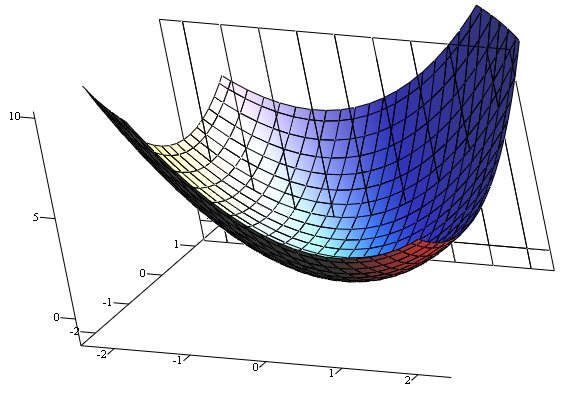
\includegraphics[scale=0.35]{3d_graph_x2+xy+y2.png}   %以pic.jpg的0.4倍大小输出
		\end{minipage}
	}
	\subfigure[$f(x,y)=x^2+xy+y^2$在$y=1$的截面图] %第二张子图
	{
		\begin{minipage}{7cm}
			\centering      %子图居中
			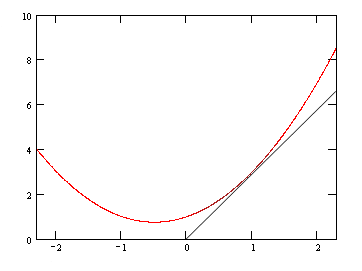
\includegraphics[scale=0.5]{X2+x+1.png}   %以pic.jpg的0.4倍大小输出
		\end{minipage}
	}
	\caption{函数$f(x,y)=x^2+xy+y^2$的3D图像和截面图} %大图名称
	%\label{fig:1}  %图片引用标记
\end{figure}

\begin{question}[\textbf{从几何意义角度看偏导数求解?}]
    $\blacktriangleright$因为曲面上的每一点都有无穷多条切线,描述这种函数的导数相当困难。偏导数就是选择其中一条切线,并求出它的斜率。通常,最感兴趣的是垂直于$y$轴(平行于$xOz$平面)的切线,以及垂直于$x$轴(平行于$yOz$平面)的切线。\\
	$\blacktriangleright$现在,欲求出函数在点$(1,1)$的与$xOz$平面平行的切线。图中显示了函数的图像以及这个平面。左图中显示了函数在平面$y = 1$上是什么样的。我们把变量$y$视为常数,通过对方程求导,我们可以发现$f$在点$(x,y)$的导数,记为:
\begin{equation}
	\frac {\partial f}{\partial x}=2x+y
\end{equation}
于是在点的与$xOz$平面平行的切线的斜率是3,即
\begin{equation}
	\frac {\partial f}{\partial x}=3
\end{equation}
在点$(1, 1)$,或称$f$在$(1, 1)$的关于$x$的偏导数是3。
\end{question}

\subsection{方向导数Directional Derivative}
\textbf{方向导数}(Directional Derivative)是分析学特别是多元微积分中的概念。一个标量场在某点沿着某个向量方向上的方向导数,描绘了该点附近标量场沿着该向量方向变动时的\textbf{瞬时变化率}。顾名思义,\textbf{方向导数就是某个方向上的导数}。其中,\textbf{偏导数描述的就是二元函数沿着$x$轴或$y$轴方向的变化率}。
\begin{question}[\textbf{方向导数的严格定义?}]
$f:U \mapsto \mathbb {R}$,是从$\mathbb {R}^{n}$上某个开集$U$映射到实数$\mathbb {R}$的函数。给定$U$内某点$\mathbf {x} =(x_{1},\ldots ,x_{n})$,以及任意非零向量 $\mathbf {v} =(v_{1},\ldots ,v_{n})$,定义一个依赖$\mathbf {x}$跟$\mathbf {v}$且从$\mathbb {R}$映射到$\mathbb {R}$的函数:
\begin{equation}
	f_{\mathbf {v}} : t \mapsto f(\mathbf {x} +t \mathbf {v})
\end{equation}
若$f_{\mathbf {v}}$对$t$的微分在$t=0$处存在,那么可以定义$f$在点$\mathbf {x}$沿向量$\mathbf {v}$的方向导数为:
\begin{equation}
	\nabla_{\mathbf {v}}{f}(\mathbf {x})=\frac {\mathrm {d} f_{\mathbf {v}}}{\mathrm {d} t}|_{t=0}=\lim _{t\rightarrow 0} \frac {f(\mathbf {x} +t\mathbf {v})-f(\mathbf {x})}{t}
\end{equation}
针对二维函数$z=f(x,y)$,$(x,y)\in D$的情况,假设求函数$f$在$(x_0,y_0)$点沿给定的方向$\vec v = (\cos \alpha , \sin \beta)$,那么公式可以写成:
\begin{equation}
	\frac{\partial f}{\partial \vec v} (x_0, y_0)=\lim_{t \to 0^{+}} \frac{f(x_0 + t \cos \alpha, y_0 + t \sin \alpha) - f(x_0, y_0)}{t}
\end{equation}
\end{question}

\subsection{梯度Gradient}
\textbf{梯度}(Gradient)是一种关于多元导数的概括。平常的一元(单变量)函数的导数是标量值函数,而多元函数的梯度是向量值函数。\textbf{多元可微函数$f$在点$P$上的梯度,是以$f$在$P$上的偏导数为分量的列向量}。
\begin{quote}
\centering
\textbf{梯度的现实解释}
\end{quote}

\begin{enumerate}
	\item 假设有一个房间,房间内所有点的温度由一个标量场$\phi$给出的,即点$(x,y,z)$的温度是$\phi(x,y,z)$。假设温度不随时间改变。然后,在房间的每一点,该点的梯度将显示变热最快的方向。\textbf{梯度的大小将表示在该方向上变热的速率}。
	\item 考虑一座高度在$(x, y)$点是$H(x, y)$的山。$H$这一点的梯度是在该点坡度(或者说斜度)最陡的方向。\textbf{梯度的大小告诉我们坡度到底有多陡}。
	\item 梯度也可以告诉我们一个数量在不是最快变化方向的其他方向的变化速度。再次考虑山坡的例子。可以有条直接上山的路其坡度是最大的,则其坡度是梯度的大小。也可以有一条和上坡方向成一个角度的路,例如投影与水平面上的夹角为60$^\circ$。则,若最陡的坡度是40\%,这条路的坡度小一点,是20\%,也就是40\%乘以60$^\circ$的余弦。这个现象可以如下数学的表示:山的高度函数$H$的梯度\textbf{点积}一个单位向量给出表面在该向量的方向上的斜率。这称为\textbf{方向导数}。
\end{enumerate}
\textbf{因此,梯度方向就是函数值增加最快的方向!!}
\begin{info}[Notice:]
	就像一元函数的导数表示这个函数图形的切线的斜率,如果多元函数在点$P$上的梯度不是零向量,则它的方向是这个函数在$P$上最大增长的方向、而它的量是在这个方向上的增长率。
\end{info}

\begin{question}[\textbf{梯度的计算?}]
标量函数 $f \colon \mathbb {R} ^{n}\mapsto \mathbb {R}$的梯度表示为:$\nabla f $或$\operatorname {grad} f$,其中$\nabla$(nabla)表示\textbf{向量微分算子}。函数$f$的梯度,$\nabla f$为向量场且对任意单位向量$\vec v$满足下列方程:
\begin{equation}
	{\big (} \nabla f(x) {\big )} \cdot \vec v =D_{\vec v} f(x)
\end{equation}
$\divideontimes$\textbf{梯度在直角坐标系中的计算}\\
$\nabla f$在三维直角坐标系中表示为:
\begin{equation}
	\nabla f={\begin{pmatrix}{\frac {\partial f}{\partial x}},{\frac {\partial f}{\partial y}},{\frac {\partial f}{\partial z}}\end{pmatrix}}={\frac {\partial f}{\partial x}}\vec i +{\frac {\partial f}{\partial y}}\vec j +{\frac {\partial f}{\partial z}}\vec k
\end{equation}其中$\vec i$, $\vec j$, $\vec k$为标准的单位向量,分别指向$x$,$y$跟$z$坐标的方向。虽然使用坐标表达,但结果是在正交变换下不变,从几何的观点来看,这是应该的。
举例来讲,函数$ f(x,y,z)=2x+3y^{2}-\sin(z)$的梯度为:
\begin{equation}
	\nabla f={\begin{pmatrix}{2},{6y},{-\cos(z)}\end{pmatrix}}=2\vec i +6y\vec j -\cos(z)\vec k
\end{equation}
\end{question}

\subsection{实值函数相对于向量和矩阵的梯度}
相对于$n \times 1$向量$\boldsymbol {x}$的梯度算子记作$\nabla_{\boldsymbol{x}}$,定义为:
\begin{equation}
	 \nabla _{\boldsymbol {x}}\overset {\mathrm {def}}{=}[\frac{\partial}{\partial x_1}, \frac{\partial}{\partial x_2}, \ldots, \frac{\partial}{\partial x_n}]^{T}=\frac{\partial}{\partial \boldsymbol{x}}
\end{equation}
\begin{enumerate}
	\item \textbf{对向量的梯度}\\
	$\blacktriangleright$以$n \times 1$实向量$\boldsymbol {x}$为变元的实标量函数$f(\boldsymbol {x})$相对于$\boldsymbol {x}$的梯度为一$n \times 1$列向量$\boldsymbol {x}$,定义为:
	\begin{equation}
		\nabla _{\boldsymbol {x}}f(\boldsymbol {x}) \overset {\mathrm {def}}{=}[\frac{\partial f(\boldsymbol {x})}{\partial x_1}, \frac{\partial f(\boldsymbol {x})}{\partial x_2}, \cdots, \frac{\partial f(\boldsymbol {x})}{\partial x_n}]^{T}=\frac{\partial f(\boldsymbol {x})}{\partial \boldsymbol{x}}
	\end{equation}
	$\blacktriangleright m$维行向量函数\( {\boldsymbol {f}}({\boldsymbol {x}})=[f_{1}({\boldsymbol {x}}),f_{2}({\boldsymbol {x}}),\cdots ,f_{m}({\boldsymbol {x}})]\)相对于$n$维实向量$n$的梯度为一$n \times m$矩阵,定义为:
	\begin{equation}
		\nabla _{\boldsymbol {x}}\boldsymbol{f}(\boldsymbol {x}) \overset {\mathrm {def}}{=}\left[
		\begin{matrix}
			\frac{\partial f_1(\boldsymbol {x})}{\partial x_1}&\frac{\partial f_2(\boldsymbol {x})}{\partial x_1}&\cdots &\frac{\partial f_m(\boldsymbol {x})}{\partial x_1}\\
			\frac{\partial f_1(\boldsymbol {x})}{\partial x_2}&\frac{\partial f_2(\boldsymbol {x})}{\partial x_2}&\cdots &\frac{\partial f_m(\boldsymbol {x})}{\partial x_2}\\
			\vdots & \vdots & \cdots & \vdots\\
			\frac{\partial f_1(\boldsymbol {x})}{\partial x_n}&\frac{\partial f_2(\boldsymbol {x})}{\partial x_n}&\cdots &\frac{\partial f_m(\boldsymbol {x})}{\partial x_n}
		\end{matrix}
		    \right]=\frac{\partial \boldsymbol{f}(\boldsymbol {x})}{\partial \boldsymbol{x}}
	\end{equation}在\textbf{向量分析}中,上述矩阵也被称为\textbf{雅可比矩阵}(也称作Jacobi矩阵,英语:Jacobian Matrix)是函数的一阶偏导数以一定方式排列成的矩阵。雅可比矩阵的其他常用符号还有:
$Df$、 $\mathrm {D} \mathbf {f}$、$\mathbf {J} _{\mathbf {f} }(x_{1},\ldots ,x_{n})$ 或者${\frac {\partial (f_{1},\ldots ,f_{m})}{\partial (x_{1},\ldots ,x_{n})}}$。
此矩阵的第$i$行是由函数$f_{i}$的梯度所表示的,$ 1 \leqslant i \leqslant m$ 。

当其为方形矩阵时,其行列式称为\textbf{雅可比行列式}(Jacobi Determinant)。Jacobi行列式的绝对值一般反映了映射函数的放大或者缩小。
	\item \textbf{对矩阵的梯度}\\
	\textbf{标量函数}$f(\boldsymbol{A})$相对于$m \times n$实矩阵$\boldsymbol{A}$的梯度为一$m \times n$矩阵,简称\textbf{梯度矩阵},定义为:
	\begin{equation}
		\nabla _{\boldsymbol {A}}\boldsymbol{f}(\boldsymbol {A}) \overset {\mathrm {def}}{=}\left[
		\begin{matrix}
			\frac{\partial f(\boldsymbol {A})}{\partial a_{11}}&\frac{\partial f(\boldsymbol {A})}{\partial a_{12}}&\cdots &\frac{\partial f(\boldsymbol {A})}{\partial a_{1n}}\\
			\frac{\partial f(\boldsymbol {A})}{\partial a_{21}}&\frac{\partial f(\boldsymbol {A})}{\partial a_{22}}&\cdots &\frac{\partial f(\boldsymbol {A})}{\partial a_{2n}}\\
			\vdots & \vdots & \cdots & \vdots\\
			\frac{\partial f(\boldsymbol {A})}{\partial a_{m1}}&\frac{\partial f(\boldsymbol {A})}{\partial x_{m2}}&\cdots &\frac{\partial f(\boldsymbol {A})}{\partial a_{mn}}
		\end{matrix}
		    \right]=\frac{\partial \boldsymbol{f}(\boldsymbol {A})}{\partial \boldsymbol{A}}
	\end{equation}
\end{enumerate}
\begin{quote}
	\textbf{更多关于矩阵求导的可以认真学习这个网址:}\href{https://zhuanlan.zhihu.com/p/29742646}{https://zhuanlan.zhihu.com/p/29742646} 
\end{quote}


%----------------------------------------------------------------------------------------
\begin{thebibliography}{2}  
\bibitem{ref1}维基百科(Wikipedia).https://zh.wikipedia.org/wiki/Wikipedia/\%E9\%A6\%96\%E9\%A1\%B5
\bibitem{ref2}陈纪修,於崇华,金路. 数学分析第二版[M].北京市:高等教育出版社,2018:33-131(上册),135-148(下册)
\end{thebibliography}
\end{document}
